% !TeX program = xelatex
%%%%%%%%%%%%%%%%%%%%%%%%%%%%%%%%%%%%%%%%%%%%%%%%%%%%%%%%%%%%%%%%%%%%%%%%%%%%%%%%
%2345678901234567890123456789012345678901234567890123456789012345678901234567890
%        1         2         3         4         5         6         7         8

\documentclass[letterpaper, 10 pt, conference]{ieeeconf}  % Comment this line out if you need a4paper

%\documentclass[a4paper, 10pt, conference]{ieeeconf}      % Use this line for a4 paper

\IEEEoverridecommandlockouts                              % This command is only needed if 
                                                          % you want to use the \thanks command

\overrideIEEEmargins                                      % Needed to meet printer requirements.

%In case you encounter the following error:
%Error 1010 The PDF file may be corrupt (unable to open PDF file) OR
%Error 1000 An error occurred while parsing a contents stream. Unable to analyze the PDF file.
%This is a known problem with pdfLaTeX conversion filter. The file cannot be opened with acrobat reader
%Please use one of the alternatives below to circumvent this error by uncommenting one or the other
%\pdfobjcompresslevel=0
%\pdfminorversion=4

% See the \addtolength command later in the file to balance the column lengths
% on the last page of the document

% The following packages can be found on http:\\www.ctan.org
%\usepackage{graphics} % for pdf, bitmapped graphics files
%\usepackage{epsfig} % for postscript graphics files
%\usepackage{mathptmx} % assumes new font selection scheme installed
%\usepackage{times} % assumes new font selection scheme installed
%\usepackage{amsmath} % assumes amsmath package installed
%\usepackage{amssymb}  % assumes amsmath package installed

\usepackage{iftex}
\ifPDFTeX
  \usepackage[utf8]{inputenc}
  \usepackage[T1]{fontenc}
\else
  \usepackage{fontspec}
  \usepackage{xeCJK}
  \setCJKmainfont{Songti SC}
  \setCJKsansfont{Heiti SC}
  \setCJKmonofont{Songti SC}
  \XeTeXlinebreaklocale "zh"
  \XeTeXlinebreakskip=0pt plus 1pt
\fi
\usepackage{amsmath,amssymb}
\usepackage{graphicx}
\usepackage{booktabs}
\usepackage{xcolor}
\usepackage{cite}
\usepackage{hyperref}
\usepackage{url}
\usepackage{microtype}
\usepackage{algorithm}
\usepackage{algorithmic}
\usepackage{multirow}
\usepackage{balance}
\usepackage{tabularx}
\usepackage{array}


\title{\LARGE \bf
Preparation of Papers for IEEE Sponsored Conferences \& Symposia*
}


\author{Albert Author$^{1}$ and Bernard D. Researcher$^{2}$% <-this % stops a space
\thanks{*This work was not supported by any organization}% <-this % stops a space
\thanks{$^{1}$Albert Author is with Faculty of Electrical Engineering, Mathematics and Computer Science,
        University of Twente, 7500 AE Enschede, The Netherlands
        {\tt\small albert.author@papercept.net}}%
\thanks{$^{2}$Bernard D. Researcheris with the Department of Electrical Engineering, Wright State University,
        Dayton, OH 45435, USA
        {\tt\small b.d.researcher@ieee.org}}%
}


\begin{document}



\maketitle
\thispagestyle{empty}
\pagestyle{empty}


%%%%%%%%%%%%%%%%%%%%%%%%%%%%%%%%%%%%%%%%%%%%%%%%%%%%%%%%%%%%%%%%%%%%%%%%%%%%%%%%
\begin{abstract}

This electronic document is a ÒliveÓ template. The various components of your paper [title, text, heads, etc.] are already defined on the style sheet, as illustrated by the portions given in this document.

\end{abstract}


%%%%%%%%%%%%%%%%%%%%%%%%%%%%%%%%%%%%%%%%%%%%%%%%%%%%%%%%%%%%%%%%%%%%%%%%%%%%%%%%
\section{INTRODUCTION}

宽视场中心相机，如鱼眼相机，能够在单幅图像中覆盖更大的场景角度范围，为视觉里程计、三维重建等几何
视觉任务提供更广的场景可见范围。然而，额外的视场只有在像素位置与空间入射射线之间的映射得到准确估
计时，才能转化为可靠的几何信息。与普通视场相机相比，宽视场相机标定主要面临两方面困难：一方面，其
投影模型具有更强的非线性，对模型选择、参数初始化和非线性优化提出了更高要求；另一方面，视场外围显
著的投影变化和图像形变增加了标定目标检测与特征定位的难度。因此，现有研究主要沿两条互补路线展开，
即改进宽视场相机模型及其参数求解，以及提高标定特征和输入观测的质量。

本文主要关注后一条路线，并从平面标定目标所提供的观测约束出发。通常，相机标定通过已知几何的平面标定目标，并根据目
标特征的图像位置估计相机内参和位姿。棋盘格和Aprilgrid
等单平面标定板因结构简单、特征易于识别而被广泛使用。在ordinary lenses下，通过平移和旋转单板标定板，
可以获得足够的观测以约束相机模型。对于wide-angle lenses，情况则更加困难。其投影模型具有较强的非线性，
标定的稳定性高度依赖可靠的初始化。当观测仅覆盖有限的径向范围，焦距尺度与畸变系数可能会产生相似的像素变化，使得这些参数难以分离，
并导致病态的线性化更新。这表明，大视场标定不仅需要足够数量的特征，还需要观测跨越不同径向区域，从而为焦距与投影模型参数提供更具区分力的几何约束。

然而，利用单块连续平面目标同时获得广泛的图像域覆盖和可靠的局部观测并不容易，其径向覆盖受到目标投影范围的限制。扩大目标的投
影范围虽然能够增加径向跨度，但也会使同一目标跨越投影变化更强的区域，对特征检测和亚像素定位提出更高要求。已有宽
视场标定研究表明，严重畸变会降低传统目标检测与特征精化的可靠性，而借助中间相机模型进行目标重投影和自适应精化
可以恢复更多有效观测。 因此，单板采集面临径向覆盖与观测可靠性之间的实际权衡，需要一种能够在不同视场区域布置可
靠观测、同时保持局部检测稳定性的标定框架。

Building on this analysis, 我们采用多个具有唯一编码的单
AprilTag 板作为可独立识别的标定单元，并将其分布在不同视场
和径向区域。与特征集中在单一连续目标区域内的棋盘格或
AprilGrid 不同，该设计允许多块标定板在同一幅图像中被独立
检测和关联，从而扩大观测的空间与径向覆盖，而无须依赖一个
连续的大尺寸目标跨越多个强投影变化区域。


单个 AprilTag 只能提供四个稀疏角点，本文将其记为
Outer4。我们首先使用大分布式的 Outer4 初始化得到
的 intermediate camera model、帧位姿和板间几
何。随后，利用该中间模型在 viewin
g-ray domain 中构造 Tag 平面内部晶格点的初始位置，并结合局部图像信息进行定位和 refinement。由此，
最终，两类观测被共同纳入统一的多板 Bun
dle Adjustment：分布式 Outer4 提供跨视场的广域支撑并建立可靠的
初始几何，而恢复的内部格点进一步密化各局部目标区域中的几何约束，共
同支持宽视场投影模型的可靠细化。基于这一方法，我们构建了一个面向宽视
场中心相机的完整多板标定系统，将多板检测与关联、内部观测恢复以及联合参数优化集成到统一流程中。

Our main contributions are summarized as follows:

\begin{itemize}
\setlength{\itemsep}{1pt}
\setlength{\parskip}{0pt}
\setlength{\parsep}{0pt}
\item We present an open-source, easy-to-deploy, and flexible multi-board
calibration system for wide-angle central cameras.
\item To address insufficient spatial coverage of calibration observations and unreliable feature refinement, we propose a distributed multi-board design based on single AprilTags, together with an intermediate-model-assisted internal lattice-point refinement method. On the evaluated sequence, the distributed design improves occupied-grid coverage by $14.6$ percentage points under the same frame--board budget.
\item 我们在相同的 Outer4 初始化条件下，通过受控分析隔离恢复的内部格点观测所带来的作用。
结果表明，局部观测密化能够提供互补约束，使宽视场投影模型得到更准确、更加符合真实几何的估计。
\end{itemize}

Tests on several datasets and camera models cover reprojection error, ablations,
cross-backend calibration, and held-out pose estimation. The results show
reliable calibration and competitive accuracy.

\section{相关工作}

\subsection{宽视场相机模型与标定}

准确的宽视场相机标定需要采用能够在较大入射角范围内保持有效的成像模型。
现有鱼眼相机和中心全向相机模型大致可以分为紧凑的参数化模型和更为灵活的
通用模型。具有代表性的参数化模型包括视场角
（Field-of-View, FOV）模型~\cite{devernay2001straight}、
Kannala--Brandt（KB）模型~\cite{kannala2006generic}、
统一相机模型~\cite{mei2007single}、
扩展统一相机模型~\cite{khomutenko2016enhanced}，
以及双球面（Double Sphere, DS）模型~\cite{usenko2018double}。
这些模型使用少量参数描述非线性的宽视场投影，因此便于参数估计和下游应用。
相比之下，通用模型通过引入更多自由度，更准确地表示复杂的镜头特性
~\cite{scaramuzza2006flexible},
~\cite{schops2020having},
~\cite{ramalingam2016unifying}。
然而，这种灵活性也提高了模型对标定观测信息量的要求。

为在实际应用中估计上述模型，研究人员开发了多种标定工具和框架。
OpenCV~\cite{bradski2000opencv} 提供了标准的鱼眼相机标定和图像校正接口；
OCamCalib~\cite{scaramuzza2006toolbox} 则利用平面棋盘格观测，
估计中心全向相机的多项式模型。
Kalibr~\cite{rehder2016extending} 在统一工具链中支持多种投影模型、
畸变模型和标定目标，并能够估计多相机系统的内参与外参。
BabelCalib~\cite{lochman2021babelcalib} 首先估计反投影模型，
再在鲁棒估计框架中回归目标正投影模型，从而改善不同中心相机模型的初始化。

即使采用灵活的相机模型和鲁棒的求解器，标定结果仍然受到观测在图像中
分布方式的影响，尤其取决于不同径向区域是否得到充分覆盖。
因此，本文关注观测构造，而不是提出新的相机模型或求解器。

\subsection{标定目标与观测构造}

基于标定目标的相机标定通常采用棋盘格、圆点阵列和编码基准标记等平面图案。
棋盘格和圆点阵列能够提供规则排列的标定点
~\cite{zhang2000flexible,heikkila2000geometric}；
AprilTag 和 ArUco 等编码标记则为每个标记赋予独立身份，
使标定目标在仅部分可见时仍能完成检测和数据关联
~\cite{olson2011apriltag,garrido2014automatic}。
此外，研究人员还设计了其他标定图案以提高特征定位精度。
例如，Deltille Grid 采用三角形平铺和局部多项式曲面拟合，
获得高精度的特征位置~\cite{ha2017deltille}。
然而，对于宽视场相机，图像外围的严重畸变仍可能降低目标检测和亚像素定位精度。

TartanCalib 利用中间相机模型重新投影 AprilTag 阵列，
并对外围特征进行精化，从而缓解上述问题
~\cite{duisterhof2022tartancalib}。
CO-Calib 从观测质量的另一个方面展开研究，并指出在内参初始化过程中，
有限的径向支撑会导致焦距尺度与鱼眼投影形状参数之间产生耦合
~\cite{liu2026observation}。

上述工作表明，可靠的局部测量和充分的径向支撑是宽视场相机标定中的
两个重要条件。这些发现促使我们构建一种灵活的框架，
将广泛的径向覆盖与密集、可靠的局部观测相结合。

\subsection{多标定板标定}

多标定板方法通常使用多个编码目标，以增强相机观测与标定目标观测之间的
几何联系。
MC-Calib~\cite{rameau2022mc} 将任意数量的基准标记图案与逐步精化过程相结合，
用于估计相机位姿和标定板位姿。
Meta-Calib~\cite{zhou2024meta} 使用单个或多个经过 ArUco 编码的
元标定板，并结合鲁棒检测和高精度标定点定位，实现相机内参与外参标定。
BabelCalib~\cite{lochman2021babelcalib} 则在鲁棒的中心相机标定框架中，
支持由多个平面标定板组成的标定目标。

现有多标定板框架主要关注稳健的目标关联、准确的标定点定位，
以及相机与标定目标几何关系的联合估计。
本文的关注点与之互补：我们利用多标定板观测构造扩大径向覆盖，
同时在每个局部标定板区域内保留密集观测。

\section{Method}

\subsection{Multi-Board Target Formulation}

Our calibration target consists of $N$ rigid boards, each carrying a
uniquely coded AprilTag:
\begin{equation}
\mathcal{B}=\{B_0,B_1,\ldots,B_{N-1}\},
\end{equation}
where $B_0$ is selected as the reference board. Let
$\mathcal{F}_{B_b}$ denote the local coordinate frame of board $B_b$,
and let $\mathbf{p}_{b,j}\in\mathbb{R}^3$ denote the $j$-th target point
expressed in $\mathcal{F}_{B_b}$. The target points include the directly
detected outer corners and the internal lattice points recovered in
Sec.~\ref{sec:internal_point_recovery}.

We use $\mathcal{F}_{B_0}$ as the common coordinate frame of the
multi-board target and fix
$\mathbf{T}_{B_0B_0}=\mathbf{I}$.
Let $\mathbf{T}_{B_0B_b}\in SE(3)$ denote the static rigid transform
from $\mathcal{F}_{B_b}$ to $\mathcal{F}_{B_0}$. For frame $t$, let
$\mathcal{F}_{C_t}$ be the camera coordinate frame and let
$\mathbf{T}_{C_tB_0}\in SE(3)$ denote the pose of the reference board
in $\mathcal{F}_{C_t}$. A point on board $B_b$ is therefore
expressed in the camera frame as
\begin{equation}
\mathbf{x}_{t,b,j}
=
\mathbf{T}_{C_tB_0}
\mathbf{T}_{B_0B_b}
\mathbf{p}_{b,j}.
\end{equation}

Given the camera parameters $\boldsymbol{\theta}$ and the projection
function $\pi(\cdot;\boldsymbol{\theta})$, the predicted image
location is
\begin{equation}
\hat{\mathbf{u}}_{t,b,j}
=
\pi\!\left(
\mathbf{x}_{t,b,j};
\boldsymbol{\theta}
\right)
=
\pi\!\left(
\mathbf{T}_{C_tB_0}
\mathbf{T}_{B_0B_b}
\mathbf{p}_{b,j};
\boldsymbol{\theta}
\right).
\end{equation}
The corresponding image observation is denoted by
$\mathbf{u}_{t,b,j}\in\mathbb{R}^2$. We collect all valid
observations in
\begin{equation}
\mathcal{O}
=
\left\{
(t,b,j,\mathbf{u}_{t,b,j})
\right\}.
\end{equation}
The unknown variables comprise the camera parameters
$\boldsymbol{\theta}$, the per-frame reference-board poses
$\{\mathbf{T}_{C_tB_0}\}$, and the static inter-board transforms
$\{\mathbf{T}_{B_0B_b}\}_{b=1}^{N-1}$.

\subsection{Camera Model Initialization}
\label{sec:camera_init}

At the beginning of calibration, no reliable camera model is available,
while a usable initialization is important for nonlinear wide-angle
calibration. The distributed AprilTag boards provide robust outer-corner
observations across different image and radial regions. We use these
observations to initialize the camera model. For a given camera-model
family, we construct an initial parameter vector
$\boldsymbol{\theta}^{0}$ using the image resolution and model-specific
default values.

For board $B_b$ observed in frame $t$, let
$\mathcal{C}^{\mathrm{out}}_{t,b}$ denote its valid outer-corner
observations. We define the reprojection residual as
\begin{equation}
\mathbf{r}^{\mathrm{out}}_{t,b,j}
(\boldsymbol{\theta},\mathbf{T})
=
\mathbf{u}_{t,b,j}
-
\pi\!\left(
\mathbf{T}\mathbf{p}_{b,j};
\boldsymbol{\theta}
\right).
\end{equation}
Given $\boldsymbol{\theta}^{0}$, a temporary frame--board pose is
initialized by
\begin{equation}
\widetilde{\mathbf{T}}^{0}_{C_tB_b}
=
\operatorname*{arg\,min}_{\mathbf{T}\in SE(3)}
\sum_{j\in\mathcal{C}^{\mathrm{out}}_{t,b}}
\left\|
\mathbf{r}^{\mathrm{out}}_{t,b,j}
(\boldsymbol{\theta}^{0},\mathbf{T})
\right\|_2^2 .
\end{equation}

We perform this initialization independently for all valid frame--board
observations and reject estimates with invalid poses or excessive
reprojection errors. Let $\mathcal{S}$ denote the retained frame--board
pairs. We then jointly refine the camera parameters and temporary poses:
\begin{equation}
\begin{aligned}
&\boldsymbol{\theta}^{*},
\left\{
\widetilde{\mathbf{T}}^{*}_{C_tB_b}
\right\}
\\
&\quad =
\operatorname*{arg\,min}_{
\boldsymbol{\theta},
\{\widetilde{\mathbf{T}}_{C_tB_b}\}}
\sum_{(t,b)\in\mathcal{S}}
\sum_{j\in\mathcal{C}^{\mathrm{out}}_{t,b}}
\rho\!\left(
\left\|
\mathbf{r}^{\mathrm{out}}_{t,b,j}
\left(
\boldsymbol{\theta},
\widetilde{\mathbf{T}}_{C_tB_b}
\right)
\right\|_2^2
\right).
\end{aligned}
\end{equation}
where $\rho(\cdot)$ is a robust loss function. At this stage, the boards
are not coupled through the unknown inter-board geometry; each valid
frame--board observation is assigned an independent pose. The optimized
parameters $\boldsymbol{\theta}^{*}$ initialize the subsequent complete
multi-board calibration and serve as the intermediate camera model for
the shared-geometry bootstrap described next.

\subsection{Shared Multi-Board Geometry Bootstrap}
\label{sec:multi_board_bootstrap}

前述相机初始化将每个 frame--board observation
视为具有独立位姿，以在未知板间布局的情况下获得稳定的中间相机模型。
然而，后续内部格点恢复需要一个统一的多板几何，以保证不同标定板上的观测
能够在同一参考坐标系下进行一致预测。
因此，在获得中间相机参数后，我们进一步利用有效的 Outer4 observations
恢复共享的刚体多板布局。

以 $B_0$ 为参考板并令
$\mathbf{T}_{B_0B_0}=\mathbf{I}$。
对于同时观测到 $B_0$ 和 $B_b$ 的已初始化帧 $t$，
由前述独立 frame--board 位姿可得到板间变换候选
\begin{equation}
\widehat{\mathbf{T}}_{B_0B_b}^{(t)}
=
\left(
\widehat{\mathbf{T}}_{C_tB_0}
\right)^{-1}
\widehat{\mathbf{T}}_{C_tB_b}.
\end{equation}
我们对同一标定板在多个共视帧中的候选进行鲁棒汇总，
得到跨帧共享的静态变换 $\mathbf{T}_{B_0B_b}$。
由此，任一局部板位姿均可统一表示为
\begin{equation}
\mathbf{T}_{C_tB_b}
=
\mathbf{T}_{C_tB_0}
\mathbf{T}_{B_0B_b}.
\end{equation}
该共享几何随后与中间相机模型共同用于
Sec.~\ref{sec:internal_point_recovery} 中内部格点的预测与恢复。

\subsection{Internal Lattice Point Recovery}
\label{sec:internal_point_recovery}

The outer corners provide stable board localization and are sufficient
to bootstrap an intermediate camera model. However, the four
observations from each tag remain locally sparse for final calibration.
We therefore use the intermediate model to recover image observations
for predefined internal lattice points, combining model-guided
prediction with local image evidence.

Given the intermediate camera parameters $\boldsymbol{\theta}^{*}$ and
the shared multi-board geometry initialized in
Sec.~\ref{sec:multi_board_bootstrap}, the direct geometric projection
of an internal lattice point
$\mathbf{p}_{b,j}$, $j\in\mathcal{C}^{\mathrm{int}}_b$, is
\begin{equation}
\widehat{\mathbf{u}}^{\mathrm{nom}}_{t,b,j}
=
\pi\!\left(
\mathbf{T}_{C_tB_0}
\mathbf{T}_{B_0B_b}
\mathbf{p}_{b,j};
\boldsymbol{\theta}^{*}
\right)
\label{eq:nominal_internal_prediction}
\end{equation}
provides a nominal prediction and is used as a fallback when the
boundary-based seed described below is unavailable.

To construct the primary seed, we sample support points along the four
observed tag boundaries and back-project them onto the unit sphere using
the intermediate camera model. The resulting top, bottom, left, and
right boundary-ray curves are denoted by
$\mathbf{r}_{T}(s)$, $\mathbf{r}_{B}(s)$,
$\mathbf{r}_{L}(t)$, and $\mathbf{r}_{R}(t)$, respectively.
Let $(s_j,t_j)\in[0,1]^2$ be the normalized horizontal and vertical
coordinates of $\mathbf{p}_{b,j}$ on the board lattice. We interpolate
the opposite boundary curves as
\begin{equation}
\begin{aligned}
\mathbf{r}_{v}
&=
\operatorname{slerp}\!\left(
\mathbf{r}_{T}(s_j),
\mathbf{r}_{B}(s_j),
t_j
\right),\\
\mathbf{r}_{h}
&=
\operatorname{slerp}\!\left(
\mathbf{r}_{L}(t_j),
\mathbf{r}_{R}(t_j),
s_j
\right).
\end{aligned}
\label{eq:spherical_boundary_interpolation}
\end{equation}
The two interpolated rays are blended and projected back to the image:
\begin{equation}
\widetilde{\mathbf{d}}^{\mathrm{int}}_{t,b,j}
=
\frac{\mathbf{r}_{v}+\mathbf{r}_{h}}
{\left\|\mathbf{r}_{v}+\mathbf{r}_{h}\right\|_2},
\qquad
\widetilde{\mathbf{u}}^{\mathrm{int}}_{t,b,j}
=
\pi\!\left(
\widetilde{\mathbf{d}}^{\mathrm{int}}_{t,b,j};
\boldsymbol{\theta}^{*}
\right).
\label{eq:internal_point_seed}
\end{equation}

Starting from $\widetilde{\mathbf{u}}^{\mathrm{int}}_{t,b,j}$, we
perform a local search in the viewing-ray domain and then refine the
candidate to subpixel accuracy in the original image. A recovered
observation is rejected if it falls outside the image, lacks sufficient
local image evidence, or deviates from its seed by more than a predefined
threshold. Each accepted observation retains its board and lattice-point
indices and is added to $\mathcal{O}$ for joint optimization together
with the outer corners.

\subsection{多板联合调整}

前述步骤依次获得中间相机模型、共享多板几何以及恢复的内部格点观测。
在最终阶段，我们在统一参考板坐标系下联合细化完整的多板标定状态
\begin{equation}
\mathcal{S}
=
\left(
\boldsymbol{\theta},
\{\mathbf{T}_{C_tB_0}\}_{t},
\{\mathbf{T}_{B_0B_b}\}_{b=1}^{N-1}
\right),
\end{equation}
其中 $\boldsymbol{\theta}$ 为相机内参，
$\mathbf{T}_{C_tB_0}$ 为第 $t$ 帧中参考板相对于相机的位姿，
$\mathbf{T}_{B_0B_b}$ 为标定板 $B_b$ 相对于参考板的静态刚体变换。
同一帧中的所有标定板共享 $\mathbf{T}_{C_tB_0}$，
而同一标定板在不同帧中的观测共享 $\mathbf{T}_{B_0B_b}$，
从而将不同帧和不同标定板上的 Outer4 与内部格点观测统一耦合到同一多板标定状态中。

对于前文定义的变换后目标点 $\mathbf{x}_{t,b,j}$，
标准图像平面重投影残差为
\begin{equation}
\mathbf{r}^{\mathrm{px}}_{t,b,j}
=
\mathbf{u}_{t,b,j}
-
\pi(\mathbf{x}_{t,b,j};\boldsymbol{\theta}).
\end{equation}
基于该残差即可完成标准的多板联合束调整。

对于宽视场相机，相同的像素偏差在不同图像位置可能对应不同的视线角偏差。
为此，我们进一步提供一种可选的球面残差形式。
给定图像观测 $\mathbf{u}_{t,b,j}$，
其归一化观测视线为
\begin{equation}
\mathbf{d}^{\mathrm{obs}}_{t,b,j}
=
\frac{
\pi^{-1}(\mathbf{u}_{t,b,j};\boldsymbol{\theta})
}{
\left\|
\pi^{-1}(\mathbf{u}_{t,b,j};\boldsymbol{\theta})
\right\|_2
},
\end{equation}
对应的预测视线为
\begin{equation}
\mathbf{d}^{\mathrm{pred}}_{t,b,j}
=
\frac{\mathbf{x}_{t,b,j}}
{\|\mathbf{x}_{t,b,j}\|_2}.
\end{equation}
令 $\mathbf{B}_{t,b,j}\in\mathbb{R}^{3\times2}$
表示 $\mathbf{d}^{\mathrm{obs}}_{t,b,j}$ 处的正交切平面基，
则局部球面残差定义为
\begin{equation}
\mathbf{r}^{\mathrm{ray}}_{t,b,j}
=
\mathbf{B}_{t,b,j}^{\top}
\left(
\mathbf{d}^{\mathrm{pred}}_{t,b,j}
-
\mathbf{d}^{\mathrm{obs}}_{t,b,j}
\right).
\end{equation}
该二维残差局部近似预测视线与观测视线之间的角度误差。

在需要同时兼顾图像平面定位与球面方向一致性时，
还可进一步采用归一化混合残差
\begin{equation}
\mathbf{r}^{\mathrm{hyb}}_{t,b,j}
=
\begin{bmatrix}
\sqrt{1-\lambda}\,
\mathbf{r}^{\mathrm{px}}_{t,b,j}/s_{\mathrm{px}}
\\
\sqrt{\lambda}\,
\mathbf{r}^{\mathrm{ray}}_{t,b,j}/s_{\mathrm{ray}}
\end{bmatrix},
\qquad
\lambda\in[0,1].
\end{equation}
其中 $s_{\mathrm{px}}$ 和 $s_{\mathrm{ray}}$
用于平衡两类残差的量纲。
$\lambda=0$ 与 $\lambda=1$ 分别退化为纯像素残差与纯球面残差。

最终联合优化可统一写为
\begin{equation}
\mathcal{S}^{*}
=
\operatorname*{arg\,min}_{\mathcal{S}}
\sum_{(t,b,j)}
w_{t,b,j}
\rho\!\left(
\left\|
\mathbf{r}_{t,b,j}(\mathcal{S})
\right\|_2^2
\right),
\end{equation}
其中 $\mathbf{r}_{t,b,j}$ 可根据具体设置选用
$\mathbf{r}^{\mathrm{px}}_{t,b,j}$、
$\mathbf{r}^{\mathrm{ray}}_{t,b,j}$
或 $\mathbf{r}^{\mathrm{hyb}}_{t,b,j}$。
有效的 Outer4 与恢复的内部格点均通过相同的残差形式共同约束相机内参、逐帧位姿和共享板间几何。

\section{EXPERIMENT}

\begin{figure}[t]
    \centering
    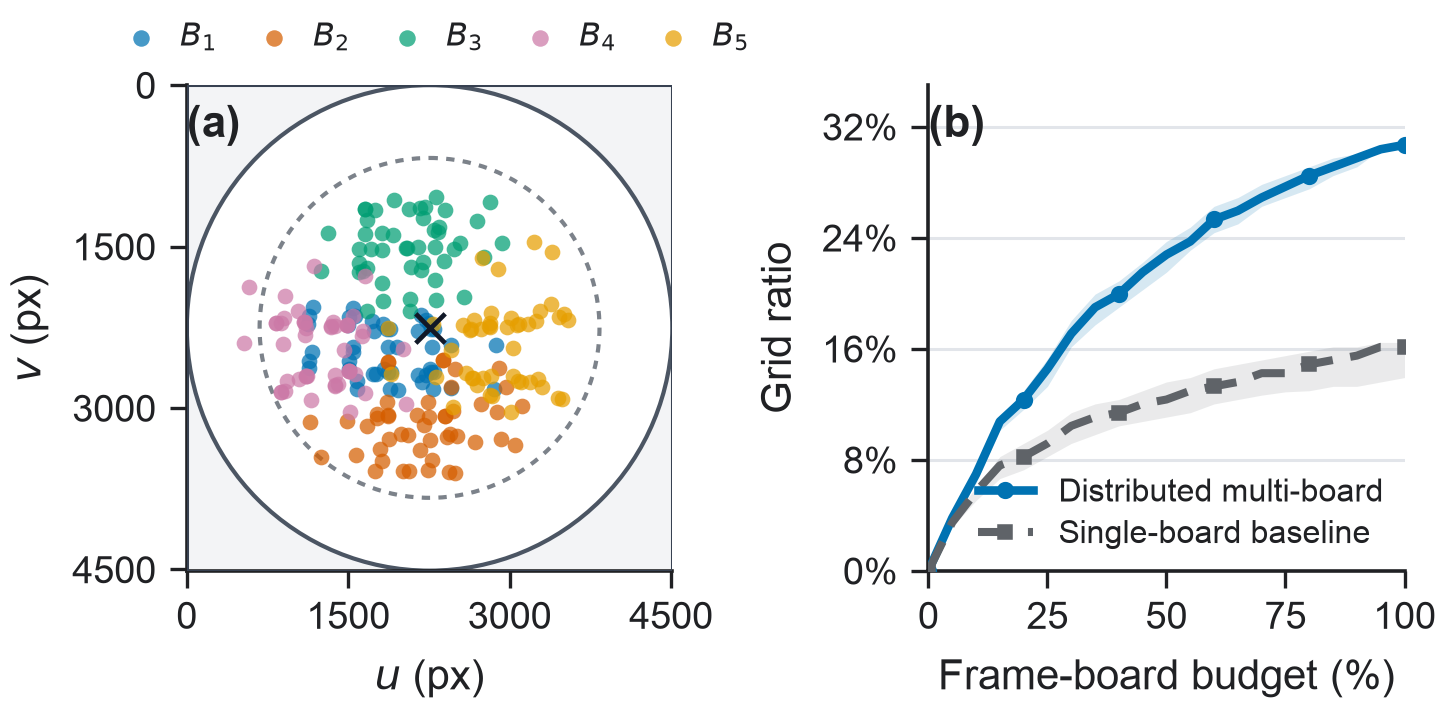
\includegraphics[width=\linewidth]{pic/corner_distribution_and_coverage_efficiency.png}
    \caption{xxxxxx}
    \label{fig:corner_distribution}
\end{figure}

\begin{table*}[t]
\centering
\caption{
Cross-backend verification on the held-out multi-board and independent
checkerboard test sets. BabelCalib uses the same detected observations
and target geometry as ours.
}
\label{tab:cross_backend_verification}

\footnotesize
\setlength{\tabcolsep}{3.2pt}
\renewcommand{\arraystretch}{1.08}

\begin{tabularx}{\textwidth}{
@{}
l
>{\raggedright\arraybackslash}p{3.75cm}
@{\hspace{1pt}}
c
c
>{\centering\arraybackslash}X
c
c
@{}
}
\toprule
\multirow{2}{*}{Model}
& \multirow{2}{*}{Method / Observations}
& \multirow{2}{*}{$f_u / f_v$}
& \multirow{2}{*}{$c_u / c_v$}
& \multirow{2}{*}{Model Params.}
& \multicolumn{2}{c}{Test RMSE [px] $\downarrow$} \\
\cmidrule(lr){6-7}
&
&
&
&
& Multi-board
& Checkerboard \\
\midrule

\multirow{3}{*}{DS}
& Ours
& 1175.65 / 1175.29
& 2242.88 / 2275.61
& $[-0.1905,\ 0.6171]$
& \textbf{0.5228}
& \textbf{0.5918} \\

& BabelCalib w/ Outer+Internal
& 1176.56 / 1175.92
& 2242.90 / 2275.63
& $[-0.1914,\ 0.6175]$
& 0.5293
& 0.6020 \\

& BabelCalib w/ Outer4 only
& 1943.49 / 1943.08
& 2242.91 / 2275.67
& $[0.3401,\ 0.8048]$
& $0.5256^{\dagger}$
& -- \\

\midrule

\multirow{3}{*}{KB}
& Ours
& 1451.58 / 1451.10
& 2242.37 / 2275.38
& $[-0.0197,\ 0.0010,\ -0.0032,\ 0.0006]$
& \textbf{0.5216}
& \textbf{0.5960} \\

& BabelCalib w/ Outer+Internal
& 1454.52 / 1453.74
& 2242.91 / 2275.65
& $[-0.0196,\ -0.0018,\ -0.0007,\ -0.0001]$
& 0.5286
& 0.6052 \\

& BabelCalib w/ Outer4 only
& --
& --
& --
& --
& -- \\

\bottomrule
\end{tabularx}

\vspace{2pt}
\parbox{\textwidth}{
\scriptsize
$^\dagger$ The Outer4-only setting achieves a comparable multi-board
test RMSE but converges to a substantially shifted intrinsic parameterization.
}
\end{table*}

\begin{table}[t]
\centering
\caption{Internal-seed ablation with a shared Outer4 initialization.}
\label{tab:internal_seed_ablation}
\footnotesize
\setlength{\tabcolsep}{1.5pt}
\renewcommand{\arraystretch}{1.05}
\begin{tabular}{@{}lcccc@{}}
\toprule
Method
& \shortstack{Reproj.\\[-1pt]Err. [px] $\downarrow$}
& \shortstack{Outer\\[-1pt]Err. [px] $\downarrow$}
& \shortstack{Internal\\[-1pt]Err. [px] $\downarrow$}
& \shortstack{Max.\\[-1pt]Err. [px] $\downarrow$} \\
\midrule
Outer-only & 0.5251 & \textbf{0.1002} & 0.5582 & 1.679 \\
Virtual Pinhole Patch & 4.3647 & 0.1089 & 4.6499 & 50.353 \\
\textbf{Spherical Seed} & \textbf{0.5243} & 0.1030 & \textbf{0.5572} & \textbf{1.678} \\
\bottomrule
\end{tabular}
\vspace{2pt}
\parbox{\columnwidth}{\scriptsize \textit{Note.} Spherical Seed is our method. Internal error uses frozen validation points excluded from Outer-only optimization; max. error is the maximum frame--board RMSE.}
\end{table}

Use this sample document as your LaTeX source file to create your document. Save this file as {\bf root.tex}. You have to make sure to use the cls file that came with this distribution. If you use a different style file, you cannot expect to get required margins. Note also that when you are creating your out PDF file, the source file is only part of the equation. {\it Your \TeX\ $\rightarrow$ PDF filter determines the output file size. Even if you make all the specifications to output a letter file in the source - if your filter is set to produce A4, you will only get A4 output. }

It is impossible to account for all possible situation, one would encounter using \TeX. If you are using multiple \TeX\ files you must make sure that the ``MAIN`` source file is called root.tex - this is particularly important if your conference is using PaperPlaza's built in \TeX\ to PDF conversion tool.

\subsection{Experimental Setup}


\subsection{Ablation}
本节分别考察内部格点观测的生成可靠性及其对相机标定的约束作用：前者比较不同 internal-seed 构造域，后者在控制初始化与观测前缀后，分析内部格点能否改善内参恢复。
\subsubsection{Internal Seed Generation}
在得到准确的外四角点的前提下，内部格点的细化依赖于初始 seed 的几何位置。我们比较 Virtual Pinhole Patch 与
Spherical Seed 两种生成方式：前者借鉴 TartanCalib 利用中间相机模型将宽视场图像重映射至虚拟针孔视图、以辅助高畸变区域特征处理的思路。
后者在 viewing-ray domain 中通过 spherical interpolation 生成 seed。两种设置共享相同的
Outer4 初始化、局部细化和优化后端，表中同时列出不恢复内部格点的 Outer-only 基线。

表~\ref{tab:internal_seed_ablation} 给出了结果。Virtual Pinhole Patch 的 outer error
与 Spherical Seed 接近，但 internal error 和 maximum error 明显增大，并导致整体
重投影误差恶化。这表明退化主要来自不可靠的内部 seed，而非 Outer4 检测或初始化。相比之下，Spherical Seed 在加
入内部观测后仍保持与 Outer-only 相近的整体误差，说明 viewing-ray-domain 构造能够
生成与宽视场投影几何一致的内部观测。

\subsubsection{Internal Observation Evaluation}
上一小节已验证 Spherical Seed 可恢复可靠的内部观测。由于它与 Outer-only 共享相同的 Outer4
初始化，两种设置均从接近收敛的模型出发，最终重投影误差难以单独反映内部格点对内参恢复的作用。
为使这一作用可被直接评价，我们令两种设置从完全相同的受扰初值出发，并比较其在相同观测条件下对初始模型偏差的约束能力。
为此，我们在 DS 模型下构造受控的内参恢复实验：令两种设置从相同的受扰初值出发，直接比较其校正
初始模型偏差的能力。两者共享参考场景、相同的 Outer4 frame--board observations 和配对噪声；唯一差别是
Outer+Internal 加入由 Spherical Seed 恢复的内部格点。

宽视场标定中，有限的径向观测可能使焦距尺度与投影形状参数产生相近的残差变化。为避免任意扰动单个内参，
我们从完整 Outer-only 观测的 pose-eliminated Schur 信息矩阵中提取最弱约束方向 $\mathbf d_{W_1}$，
并将其固定用于两种设置和全部观测预算。对于方法 $m$ 和预算 $b$，沿该方向的总信息定义为
\begin{equation}
I_{W_1}^{m,b}=
\mathbf d_{W_1}^{\top}\mathbf S_c^{m,b}\mathbf d_{W_1},
\end{equation}

随后，我们沿该方向扰动参考 DS 内参，使初始模型在外围区域 $\rho\geq0.7$ 的 Ray Error P95
为 $2^\circ$。图~\ref{fig:internal-point-ablation} 分别考察弱方向约束、全视场模型恢复误差和
达到外围精度目标所需的观测预算。

\begin{figure*}[t]
  \centering
  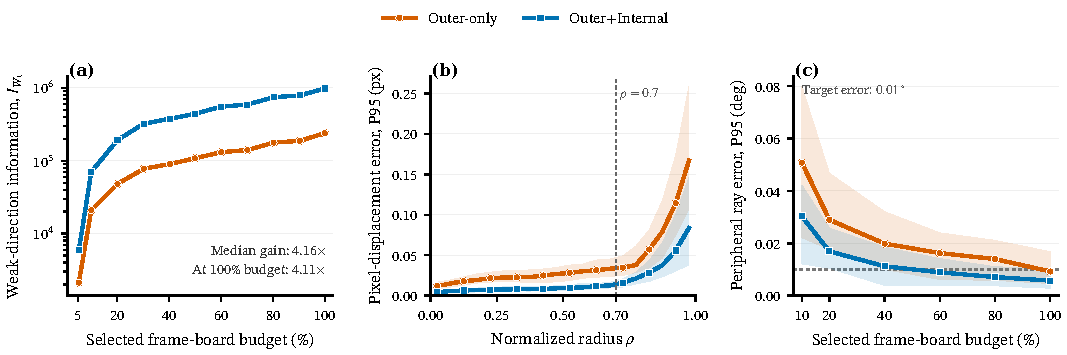
\includegraphics[width=0.98\textwidth]{pic/internal_point_ablation.pdf}
  \caption{内部观测对受扰 DS 内参恢复的影响。Outer-only 与
  Outer+Internal 共享相同的 Outer4 frame--board observations、
  受扰初值和配对噪声；Outer+Internal 仅额外加入恢复的内部格点。
  (a) 消除位姿后的最弱内参方向 $W_1$ 上的 Schur 信息。
  (b) 在固定参考射线网格上计算的、恢复模型相对参考模型的径向像素
  位移 P95。(c) 不同 frame--board 预算下的外围 Ray Error P95。
  两种设置均从 $2^\circ$ 外围扰动出发，并仅优化 DS 内参。
  图 (b) 和 (c) 汇总 100 组配对试验，曲线和阴影分别表示中位数和
  IQR；外围区域定义为 $\rho \geq 0.7$。}
  \label{fig:internal-point-ablation}
\end{figure*}

如图~\ref{fig:internal-point-ablation}(a) 所示，加入内部格点后，在全部 frame--board
预算下均获得更强的弱方向约束。图~\ref{fig:internal-point-ablation}(b) 显示，恢复模型在全视场
内更接近参考模型，且改善在图像外围更明显。图~\ref{fig:internal-point-ablation}(c) 给出一致的
预算趋势：Outer+Internal 以更少的观测预算达到预设的外围精度目标。这些结果表明，内部格点不替代
分布式 Outer4 提供的初始化，而是在其基础上补充局部约束，从而改善高畸变外围区域的 DS 模型恢复。

\subsection{Camera Pose Estimation}

为了评估标定结果在未见观测上的几何泛化能力，我们在 held-out
test images 上进行相机位姿估计，并将数据随机划分为 $7{:}3$ 的
训练集和测试集。对于每种方法，测试阶段固定待评价的相机内参和统一的
多板目标几何，仅通过鲁棒重投影优化估计每帧参考板到相机的位姿。
随后，在该帧所有可见的 board 观测上计算重投影误差，并采用 RMSE、
P95 和 Inlier@1px 作为评价指标。

由于对照的基线方法的原生流程无法直接适配本文的多板标定场景，我们使用
标准棋盘格标定流程估计相机内参，再将所得内参与本文方法置于相同的
held-out 多板位姿估计任务中进行参考性对比。

\subsection{Camera Pose Estimation}

为评估本文观测构造的跨后端适用性，我们将前端生成的同一组
Outer4+Internal 二维--三维对应关系导出至 BabelCalib，并分别
估计 Double Sphere（DS）和 Kannala--Brandt（KB）模型。随后，
将所得标定结果与本文标定流程在相应模型下的结果进行比较。如表所示，
对于两种相机模型，两个后端在留出多板数据集和棋盘格数据集上均取得了
相近的重投影均方根误差，且所有配置均获得了有效的标定结果。这表明，
本文构造的观测能够被不同的标定后端有效利用，并适用于不同的宽视场投影模型。

\subsection{Downstream}

为评价标定结果在未参与标定的场景图像中的双目几何一致性，我们使用由两台 Allied Vision 相机构成的双目系统，分别开展外围极线一致性评价和 StereoSGBM 视差实验，用于考察大视场区域的跨视图几何及标定结果对稠密双目匹配的影响。


表~X 报告整体误差中位数，以及外围区域（θ≥60）的中位数和 P95。图~X 在原
始鱼眼图像中展示中心、中间和外围区域的六个固定匹配点，其中曲线、叉号和空心
圆分别表示预测极线、实际匹配位置和极线最近点。结果用于评价分布式多板和内部格
点观测能否改善大极角区域的双目几何。

\begin{table}[t]
  \centering
  \caption{Cross-backend evaluation on the held-out multi-board and
  checkerboard datasets. Lower is better.}
  \label{tab:cross_backend}
  \small
  \setlength{\tabcolsep}{3.5pt}
  \renewcommand{\arraystretch}{1.08}
  \begin{tabular}{@{}llcc@{}}
    \toprule
    \multirow{2}{*}{Camera}
    & \multirow{2}{*}{Model}
    & \multicolumn{2}{c}{Reproj.Err. [px] } \\
    \cmidrule(lr){3-4}
    & & Multi-board & Checkerboard \\
    \midrule
    Action Pro & DS & -- & -- \\
    Alvium U-2040m & DS & 0.7047 & 0.5816 \\
    Alvium U-2040m & KB & 0.7031 & 0.5815 \\
    \bottomrule
  \end{tabular}
\end{table}

\begin{table*}[t]
  \centering
  \caption{Reprojection performance on two held-out multi-board sets and one checkerboard set. Metrics are reported as RMSE [px], P95 [px], and Inlier@1px [\%].}
  \label{tab:reprojection_comparison}
  \scriptsize
  \renewcommand{\arraystretch}{1.06}
  \setlength{\tabcolsep}{2.6pt}
  \begin{tabular*}{\textwidth}{@{\extracolsep{\fill}}clccccccccc@{}}
  \toprule
  \multirow{2}{*}{Model} & \multirow{2}{*}{Method}
  & \multicolumn{3}{c}{Multi-Board Set 1}
  & \multicolumn{3}{c}{Multi-Board Set 2}
  & \multicolumn{3}{c}{Checkerboard Set} \\
  \cmidrule(lr){3-5}\cmidrule(lr){6-8}\cmidrule(lr){9-11}
  & & RMSE $\downarrow$ & P95 $\downarrow$ & Inl. $\uparrow$
    & RMSE $\downarrow$ & P95 $\downarrow$ & Inl. $\uparrow$
    & RMSE $\downarrow$ & P95 $\downarrow$ & Inl. $\uparrow$ \\
  \midrule
  \multirow{4}{*}{DS}
  & \textbf{Ours}       & \textbf{0.523} & \textbf{0.990} & \textbf{95.1} & \textbf{0.634} & \textbf{1.378} & \textbf{88.2} & -- & -- & -- \\
  & Kalibr              & 0.600 & 1.093 & 92.6 & 0.806 & 1.638 & 84.2 & -- & -- & -- \\
  & TartanCalib         & 0.623 & 1.155 & 91.7 & 0.814 & 1.671 & 83.7 & -- & -- & -- \\
  & BabelCalib          & 0.618 & 1.147 & 91.7 & 0.848 & 1.682 & 83.6 & -- & -- & -- \\
  \addlinespace[2pt]
  
  \multirow{6}{*}{KB}
  & \textbf{Ours}       & \textbf{0.522} & \textbf{0.984} & \textbf{95.3} & \textbf{0.631} & \textbf{1.375} & \textbf{88.5} & -- & -- & -- \\
  & Kalibr              & 0.599 & 1.092 & 92.7 & 0.761 & 1.585 & 84.8 & -- & -- & -- \\
  & TartanCalib         & 0.619 & 1.140 & 91.8 & 0.782 & 1.595 & 84.6 & -- & -- & -- \\
  & CamOdoCal           & 0.605 & 1.119 & 92.5 & 0.763 & 1.587 & 85.0 & -- & -- & -- \\
  & BabelCalib          & 0.617 & 1.147 & 91.8 & 0.792 & 1.628 & 84.2 & -- & -- & -- \\
  & OpenCV fisheye      & 0.583 & 1.071 & 93.1 & 0.760 & 1.570 & 85.2 & -- & -- & -- \\
  \addlinespace[2pt]
  
  \multirow{6}{*}{\shortstack{UCM\\/ Mei}}
  & \textbf{Ours}       & \textbf{0.520} & \textbf{0.989} & \textbf{95.2} & \textbf{0.636} & \textbf{1.377} & \textbf{88.3} & -- & -- & -- \\
  & Kalibr              & -- & -- & -- & -- & -- & -- & -- & -- & -- \\
  & TartanCalib         & -- & -- & -- & -- & -- & -- & -- & -- & -- \\
  & CamOdoCal           & 0.605 & 1.110 & 92.6 & 0.816 & 1.645 & 83.9 & -- & -- & -- \\
  & BabelCalib          & 0.737 & 1.335 & 87.5 & 1.207 & 1.756 & 83.7 & -- & -- & -- \\
  & OpenCV omnidir      & 0.606 & 1.108 & 92.2 & 0.852 & 1.686 & 83.6 & -- & -- & -- \\
  \addlinespace[2pt]
  
  \multirow{4}{*}{EUCM}
  & \textbf{Ours}       & -- & -- & -- & -- & -- & -- & -- & -- & -- \\
  & Kalibr              & -- & -- & -- & -- & -- & -- & -- & -- & -- \\
  & TartanCalib         & -- & -- & -- & -- & -- & -- & -- & -- & -- \\
  & BabelCalib          & -- & -- & -- & -- & -- & -- & -- & -- & -- \\
  \bottomrule
  \end{tabular*}
  \end{table*}  

\section{CONCLUSIONS}

A conclusion section is not required. Although a conclusion may review the main points of the paper, do not replicate the abstract as the conclusion. A conclusion might elaborate on the importance of the work or suggest applications and extensions. 

\addtolength{\textheight}{-12cm}   % This command serves to balance the column lengths
                                  % on the last page of the document manually. It shortens
                                  % the textheight of the last page by a suitable amount.
                                  % This command does not take effect until the next page
                                  % so it should come on the page before the last. Make
                                  % sure that you do not shorten the textheight too much.

%%%%%%%%%%%%%%%%%%%%%%%%%%%%%%%%%%%%%%%%%%%%%%%%%%%%%%%%%%%%%%%%%%%%%%%%%%%%%%%%



%%%%%%%%%%%%%%%%%%%%%%%%%%%%%%%%%%%%%%%%%%%%%%%%%%%%%%%%%%%%%%%%%%%%%%%%%%%%%%%%



%%%%%%%%%%%%%%%%%%%%%%%%%%%%%%%%%%%%%%%%%%%%%%%%%%%%%%%%%%%%%%%%%%%%%%%%%%%%%%%%
\section*{APPENDIX}

Appendixes should appear before the acknowledgment.

\section*{ACKNOWLEDGMENT}

The preferred spelling of the word ÒacknowledgmentÓ in America is without an ÒeÓ after the ÒgÓ. Avoid the stilted expression, ÒOne of us (R. B. G.) thanks . . .Ó  Instead, try ÒR. B. G. thanksÓ. Put sponsor acknowledgments in the unnumbered footnote on the first page.



%%%%%%%%%%%%%%%%%%%%%%%%%%%%%%%%%%%%%%%%%%%%%%%%%%%%%%%%%%%%%%%%%%%%%%%%%%%%%%%%

References are important to the reader; therefore, each citation must be complete and correct. If at all possible, references should be commonly available publications.



\bibliographystyle{IEEEtran}
\bibliography{references}



\end{document}
